%!TEX TS-program = pdflatex                                                    %
%!TEX encoding = UTF8                                                          %
%!TEX spellcheck = en-US                                                       %
%------------------------------------------------------------------------------%
% to compile use "latexmk --pdf main.tex"                                      %
%------------------------------------------------------------------------------%
% to count words 
% "pdftotext main_nofigs_nocaptions.pdf - | egrep -e '\w\w\w+' | iconv -f ISO-8859-15 -t UTF-8 | wc -w"
% -----------------------------------------------------------------------------%

\usepackage{url}
\usepackage[english]{babel}
\usepackage[utf8]{inputenc}
\usepackage[T1]{fontenc}
%\usepackage[pdftex]{graphicx} 
%\usepackage{graphics}
%\usepackage{hyperref}
\usepackage{float}
\floatplacement{figure}{H}
\usepackage{booktabs}     % nice tables
\usepackage{tabularx}     % even nicer tabular environments 
\usepackage{amsmath}
\usepackage{amsfonts}
\usepackage{amssymb}
%\usepackage{multicol}
\usepackage{listings}
\usepackage{tikz,times}
\usepackage{courier}
\usepackage[scaled]{beramono}

\usepackage{fancyvrb}

\usetikzlibrary{shapes,arrows}
\usetikzlibrary{arrows,positioning}
\usepackage{xcolor}
\usepackage[font=bf]{subfig}
\usepackage[inline]{trackchanges}

%%%%%%% setup track changes "editors"

\addeditor{mw}
\addeditor{lp}
\addeditor{psl}
\addeditor{ld}
\addeditor{sk}
\addeditor{vj}
\addeditor{jm}

%\usepackage{sectsty}
%\sectionfont{\normalsize\bfseries}
%\usepackage[labelfont=bf]{caption}
%\usepackage{endfloat} %place figures at end of document
%------------------------------------------------------------------------------%
%\captionsetup{
%%format = hang,                % caption format
%labelformat = simple,          % caption label : name and number
%labelsep = period,             % separation between label and text
%textformat = simple,           % caption text as it is
%justification = justified,     % caption text justified
%singlelinecheck = true,        % for single line caption text is centered
%font = {up,singlespacing},     % defines caption (label & text) font
%labelfont = {bf,footnotesize}, % NOTE: tiny size is not working
%textfont = footnotesize,
%%width = \textwidth,           % define width of the caption text
%skip = 1ex,                    % skip the space between float and caption
%listformat = simple,           % in the list of floats, label + caption
%}

%------------------------------------------------------------------------------%
%\hypersetup{
%    bookmarks=true,         % show bookmarks bar?
%    unicode=false,          % non-Latin characters in Acrobat’s bookmarks
%    pdftoolbar=true,        % show Acrobat’s toolbar?
%    pdfmenubar=true,        % show Acrobat’s menu?
%    pdffitwindow=false,     % window fit to page when opened
%    pdfstartview={FitH},    % fits the width of the page to the window
%    pdftitle={TheVirtualBain},    % title
%    pdfauthor={PSL},        % author
%    pdfsubject={ProposedArticle},   % subject of the document
%    pdfcreator={paupau},    % creator of the document
%    pdfnewwindow=true,      % links in new window
%    colorlinks=true,       % false: boxed links; true: colored links
%    linkcolor=red,          % color of internal links (change box color with linkbordercolor)
%    citecolor=blue,        % color of links to bibliography
%    filecolor=magenta,      % color of file links
%    urlcolor=blue           % color of external links
%}
%-----------------------------------------------------------------------
%\usepackage{subcaption}

%%%%%%%%%%%%%%%%%%%%%%%%%%%%%%%%%%%%%%%%%%%%%%%%%%%%%%%%%%%%%%%%%%%%%%%%%%%%%%%%
%%                             New and renew commands                         %%
%%%%%%%%%%%%%%%%%%%%%%%%%%%%%%%%%%%%%%%%%%%%%%%%%%%%%%%%%%%%%%%%%%%%%%%%%%%%%%%%
  
\renewcommand{\lstlistingname}{Code}
\renewcommand{\thesubfigure}{\Alph{subfigure}}
%\newcommand{\inputTikZ}[2]{\scalebox{#1}{\input{#2}}}
\newcommand*{\h}{\hspace{5pt}}   % for indentation
\newcommand*{\hh}{\h\h}          % double indentation
\newcommand*{\tvbmodule}[1]{{\textsc{#1}}}          % scientific modules in "simulator"
\newcommand*{\tvbdatatype}[1]{\textbf{\emph{#1}}}   % datatypes in "datatypes"
\newcommand*{\tvbclass}[1]{{\ttfamily\emph{#1}}}    % classes either in simulator mods or datatypes
\newcommand*{\tvbmethod}[1]{{\textsf{#1}}}          % methods
\newcommand*{\tvbattribute}[1]{{\ttfamily{#1}}}     % attributes
\newcommand*{\tvbtrait}[1]{{\ttfamily{#1}}}         % traited types

\newcommand{\matlab}{MatLab}

%%%%%%%%%%%%%%%%%%%%%%%%%%%%%%%%%%%%%%%%%%%%%%%%%%%%%%%%%%%%%%%%%%%%%%%%%%%%%%%%
%%                            Colors and graphics                             %%
%%%%%%%%%%%%%%%%%%%%%%%%%%%%%%%%%%%%%%%%%%%%%%%%%%%%%%%%%%%%%%%%%%%%%%%%%%%%%%%%
\definecolor{palegreen}{HTML}{DAFFDA}
\definecolor{lightgray}{rgb}{0.15,0.15,0.15}
\definecolor{orange}{HTML}{FF7300}
\DeclareGraphicsExtensions{.jpg,.pdf,.png,.tiff}%,.mps,.bmp
\graphicspath{{figures/}}
 
%##--------------------------------------------------------------------------##%
%##                               START HERE                                 ##%
%##--------------------------------------------------------------------------##%
\copyrightyear{}
\pubyear{}

\begin{document}
\lstset{language=Python,
	captionpos=b,
	keepspaces=true,
	numbers=none,
	showspaces=false,
    float=*,
	basicstyle=\fontsize{8pt}{8}\ttfamily
	} 

\firstpage{1}

%%  Authorship and Title
\title[TVB]{Integrating neuroinformatics tools in TheVirtualBrain}
\author[Woodman {et~al}]{
        M. Marmaduke Woodman\,$^{1,*}$,  
        Laurent Pezard\,$^{1}$,  
        Lia Domide\,$^{3}$, 
        Stuart Knock\,$^{1}$, 
        Paula Sanz Leon\,$^{1}$, 
        Jochen Mersmann\,$^{2}$,
        Anthony R. McIntosh \,$^{4}$ and  
        Viktor Jirsa\,$^{1}$\footnote{to whom correspondence should be addressed: marmaduke.woodman@univ-amu.fr,
        viktor.jirsa@univ-amu.fr}}

\address{$^{1}$ Institut de Neurosciences des Syst{\`e}mes, Aix-Marseille
    Universit\'e,  27, Bd. Jean Moulin, 13005, Marseille, France.\\
         $^{3}$ Codemart, 13, Petofi Sandor, 400610, Cluj-Napoca, Romania.\\
         $^{2}$ CodeBox GmbH, Hugo Eckener Str. 7, 70184 Stuttgart, Germany.\\
         $^{4}$ Rotman Research Institute at Baycrest, Toronto, M6A 2E1, Ontario, Canada\\
        }

\history{}

\editor{}

\maketitle

%##--------------------------------------------------------------------------##%
%##                               ABSTRACT                                   ##%
%##--------------------------------------------------------------------------##%


\begin{abstract}
\section{}

TheVirtualBrain (TVB) is a neuroinformatics Python package representing the
convergence of lines of work in clinical, systems, theoretical neuroscience in
the integration, analysis, visualization and modeling of neural dynamics of the
human brain as well as the imaging modalities through which these dynamics are
measured. Specifically, TVB is composed of a flexible simulator for both neural
dynamics and modalities such as electroencephalography (EEG), magnetoencephalography (MEG) and functional magnetic resonance imaging (fMRI), common analysis techniques such
as wavelet decomposition and multiscale sample entropy, interactive visualizers
for replaying cortical timeseries on the 3D surface or editing large-scale
connectivity matrices, and an (optional) user interface accessible through
modern web browsers. Tying together these pieces with persistent data storage,
based on a combination of SQL \& HDF5, is a rich, open-ended system of
datatypes modeling (systems level) neuroscientific data and the relations among
them. This data modeling system in parallel with the so-called adapter pattern
architecture permit the integration of TVB with any other computational system,
including MATLAB, for which support is already available.  Notably, TVB provides
infrastructure for multiple projects and multiple users, possibly participating
under multiple roles: for instance, a clinical researcher may import structural data of a patient obtained from various techniques such as magnetic resonance imaging (MRI) or diffusion spectrum imaging (DSI) \note[sk]{Is this actually true? I'm not really
up to date on this aspect of things, but, the last time I paid attention this 
feature wasn't fully integrated/functional -- If not, then it seems like a bad 
idea to publish that something is possible when it isn't...}\note[vj]{I changed the text. done}, identify 
potential lesion points, and then
share this data with a computational expert who would then enter to contribute
simulation parameter sweeps and analyses, to test which lesion point is most
probably given certain empirical imaging data, et cetera. This is one of many
multi-user use cases supported by TVB.  TVB also drives research forward on
many levels: the simulator itself represents the systematization of several
recent ad-hoc simulations in the modeling literature on human resting state.  In
these ways, TVB serves as an integrating neuroinformatics platform for various tools and disparate expertises in the high level analysis, handling of structural and functional data and modeling of the human brain.  Here we briefly outline the history and motivation for TVB as a unified project
\textit{per se}. We proceed to describe the framework and simulator, giving
usage examples in the web UI and in plain Python scripting.  Finally, we
compare TVB with the nearest neighbors in brain modeling, simulation
performance, recent advances thereupon with native code compilation and GPUs,
and the role of Python and its rich scientific ecosystem in TVB. 

  
\section{Keywords:} large-scale brain network, simulation,  web platform, Python, virtual
brain, connectivity, connectome, neural mass, neural field, time delays,
full-brain network model, GPUs

\end{abstract}

%\tableofcontents

\note[lp]{Emphasize the process of integrating new tools in TVB? This is not
completely clear for me now.}

\section{Motivations}
Neurosciences and more generally brain and behavioral sciences imply a large
amount of interactions between scientific disciplines to fulfill their endeavour
in the comprehension of brain and behavior relationship\footnote{Several
    important scientific projects such as The Human Brain Project are clear
illustration thereof.}. Nevertheless, one major drawback of this
interdisciplinary enterprise is the necessary distribution of competences most
frequently between individuals, but also, in a non negligable number of cases,
between institutes.  Moreover, the large increase of technical demands for data
analysis and brain simulation usually prevents from an optimal diffusion of these
advances in the more experimentally oriented part of the community. 

These problems appeal at least two orientations for their solution. Firstly,  the
development of up to date computing and simulating librairies using commonly
used languages and secondly, the development of tools for sharing
competences and data. Due to the high pace of new developments, these solutions
should also remain open to incoming new tools. Several projects fall in the
first category (from Statistical Paramteric Mapping (SPM) to Brain Connectivity Toolbox, fieldtrip in the \matlab{} "galaxy"
and from "nitime" to neo... to name only a few). In the second category CARMEN
(http://www.carmen.org.uk/) G-Node (https://portal.g-node.org/data/)
\note[lp]{Other projects?} are (web) platforms for collaborative work and data
sharing.\note[vj]{clean up the names here and provide references please} .

TheVirtualBrain (TVB) provides its own solutions to these two problems.  In an
initial step, they were addressed in two independent developments: one whole
brain-simulator library developped in \matlab{} and a web platform for
collaborative interactions in the context of multi-purpose data analysis which
was developed in Python.  In each case, the choice of the language was dictated
both by the scientific context and the technical constraints. For the
integration of these preexistent tools and the radically new organization in
one integrating neuroinformatics platform, TheVirtualBrain, the final choice of
language was Python\footnote{The first issue of Python in Neurosciences also
confirmed the choice of the Python language.}, since it provides the main
technical elements: database interactions, web programming, object-oriented
programming and abstraction.

\subsection{Why another project? (TVB compared to others)}

To what degree is it possible to benefit from existing simulator platforms and
data base management architectures as opposed to developing a completely new
neuroinformatics platform? Such was the key question posed at the conception of
the TVB project. Finally, TVB was developed as a new neuroinformatics platform
with a focus on simulation, but its architecture was certainly inspired by its
predecessors.

\subsubsection{The architecture}

\note[vj]{There is no need to describe the steps that did not work, in fact it
is counter productive and distracting. I removed them from the paragraphs}

The TVB architecture was developed to allow easy integration of any
computational tools along with a system for describing typical types of data.
The two main constraints for the architecture were then to provide a web
interface to allow remote collaboration and a data exchange system to allow the
exchange of data (or simulation results) between users. Added to this that
the user interface should have a particular design, one obtains the well-known
"model-view-controller" design \note[lp]{detail this}.  We chose
\textsf{CherryPy} for the web  and \textsf{SQLAlchemy} for the database
exchanges\footnote{Other dependencies of TVB are listed in
    \texttt{TVB\_INSTALL\_REQUIREMENTS} which currently lists
    \texttt{"apscheduler", "beautifulsoup", "cherrypy", "cfflib", "formencode",
        "lxml", "minixsv", "mod\_pywebsocket", "networkx", "nibabel", "numpy",
        "numexpr", "psutil", "scikit-learn", "scipy", "simplejson",
        "sqlalchemy", "sqlalchemy-migrate"}.}

Moreover, the requirement for data visualisation impose to develop specific
modules thanks to WebGL availability in modern browsers.

The architecture of TVB had been prototyped in Python, and in turn, both the
language and the scientific ecosystem were more than rich enough to support
continued developed entirely within Python, of both the architecture and the
simulator, in addition to it being a general purpose language. Lastly, Python's
emphasis on readability and idiomatic style facilitates integration of 
code contributions from programmers with disparate backgrounds.

\note[lp]{For Lia: Was Python a "good" choice? and why? Which other language would have
done the job?}

\subsubsection{The simulator}



A significant part of TVB is simulating large-scale brain networks. While
several existing simulators could have been adapted, we have estimated that
TVB style simulations are far enough outside the design of other simulators to
make a new development necessary. We discuss the reasons thereof in the following. 

The existing neural network simulators focus first on abstract rate neurons (in
the style of PDP) and modelling neurocognitive processes, on one hand, and on
the other, full multicompartmental neuron simulators treating complex spatial
geometries, e.g. NEURON \cite{Hines_2001}.  More recently, due to interest in
the computational properties of spiking neurons and their relevance to
experimental observations, simulators targeting specifically spiking neurons
have been prominent, e.g. Brian \cite{Goodman_2009}. Initial considerations
were given to  Brian \note[lp]{cite BRIAN} since it allows for a generic
implementation of differential equations. However, special demands imposed on
large scale brain network modeling, in particular spatially distributed time
delays and stochasticity, rendered the use of BRIAN complicated and tedious.
In TVB the network nodes are defined by neural population and neural field
models \cite{Deco_2008a, Coombes_2010} rather than cellular models. Here, the
spatial extent of the modeled dynamics is far larger and hence permits networks
thereof to scale reasonably to the entire cortex, under the assumptions of the
models, when combined with empirical measurements of cortico- cortical
connectivity. Therefore, the physical scale modeled by the TVB simulators
differs from that for which other simulators were designed.  Several technical
issues stem from this scale, e.g. efficient handling of dense $N^2$ delays and
neural field-like connectivity, which will be discussed in more detail below.
Further TVB specific constraints are non-existent for previous simulators and
hence no support exists. For instance the network nodes need to be positioned
and connected within the three-dimensional physical space respecting anatomical
geometry. The transformations from the physiological signals to the commonly
used imaging modalities such as EEG, MEG and fMRI need to be employed. All
these constraints originate from the "large brain network" scale of simulation
in TVB, which is clearly different from the more usual "cellular" simulations
as typically performed by the existing neuronal network simulators. As such,
TheVirtualBrain represents the first simulator dedicated to modeling the brain
network on the full-brain scale. 


Large scale simulation implies flexible integration. We shall see
how this is enable by the architecture..
\note[mw]{expand}

\subsection{Practical informations / contributors information}

To address these concerns, a flexible architecture was developed to
allow easy integration of any computational tools along with a system
for describing typically types of data. A web based UI was developed
for users not comfortable with programming, as well as \matlab{} toolbox
for interacting with the Python based framework, given that many
neuroscientists are already comfortable with the \matlab{} workflow.

Lastly, a high performance, highly documented simulator along with
various forward solutions have been implemented and released under a
GPL licence to ensure universal access to high quality simulations, 
developed on the well-known Github, making it extremely easy for 
anyone to contribute.

TVB source code is available for download on Github at
\url{https://github.com/the-virtual-brain/}.  Previous Git and Python knowledge
is required for contributing.  Although you could independently install Python
and the rest of TVB dependencies on your machine, and then use the Github code
as a simple local clone, we recommend you to download \emph{TVB\_ Distribution}
from \url{http://www.thevirtualbrain.org/register/}, fork our repositories on
Github and further use \emph{contributor\_setup} script, from inside \emph{TVB\_Distribution} 
folder, to link the two.  In this recommended use-case, you will
have all TVB dependencies already prepared and at your disposal, as part of
\emph{TVB\_Distribution}.\note[lp]{Is there any plan for a .deb package with
full dependencies taken into account in this context? Or Pypi?} 

\note[lp]{Generic description and goal of the paper}

The overall structure of TVB is depitcted on Figure~\ref{fig:architecture} where
components of the architecture and of the scientific library are shown with
their relationships.

 \begin{figure*}
        \centering
        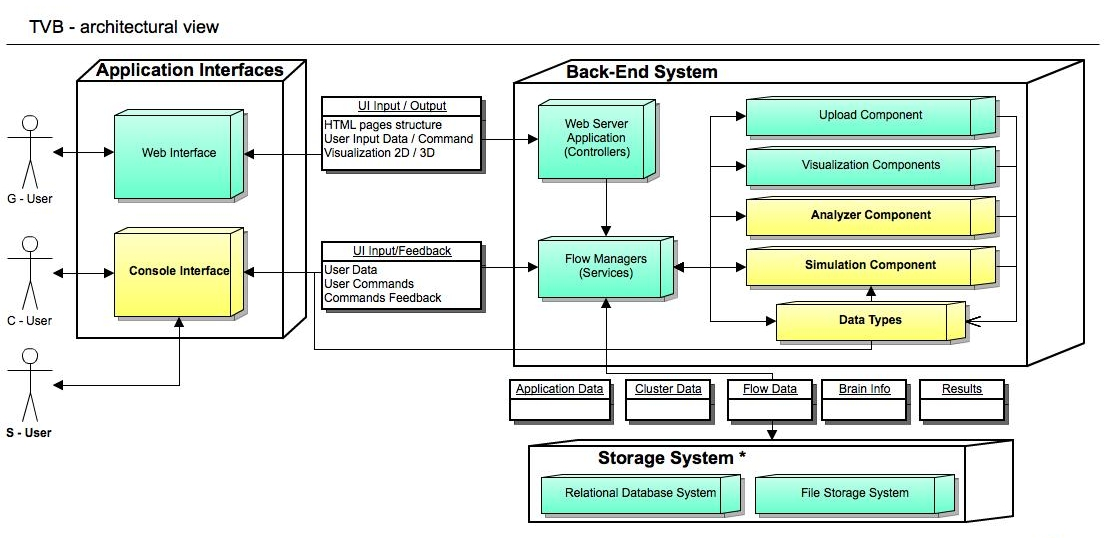
\includegraphics[width=0.90\textwidth]{images/architecture.jpg}
        \caption{TVB architecture: Yellow blocks are part of the Scientific
            Library of TVB, while the green blocks are part of TVB Framework.
            TVB provides two independent interfaces, depending on the
            interaction type wanted by the end-user (web or console).  TVB
            Storage layer is compulsory for the web interface, but it can be
            switched on/off for the console interface.  \note[lp]{It is said in
                the text that "console interface" is part of the "architecture"
            and not the "scientific library", this is the contrary on the
        figure}
        \note[lp]{What is a "S-User"? I missed the definition?}
         }
        \label{fig:architecture}
 \end{figure*}

 The goal of this article is firstly to decribre TVB framework from the
 development point of view and demonstrates how it interacts with other tools
 and how it can be extended (on the basis of extension already integrated in
 TVB).


\section{Architecture}

\TVB is logically and technically divided at deploy time into a scientific library and a framework, 
where the scientific library includes datatypes, common analyses and the simulator as its central piece,
while the framework handles execution infrastructure, the web-based user interface and database connectivity. 
While TVB Scientific Library can function independently, as a Python module, TVB Framework needs the scientific library to wrap around it at runtime.

\TVB source code is available for download on Github at \url{https://github.com/the-virtual-brain/}. Previous Git and Python knowledge is required for contributing.
Although you could independently install Python and the rest of TVB dependencies on your machine, and then use the Github code as a local clone, 
we recommend you to download TVB Distribution from \url{http://www.thevirtualbrain.org/register/}, fork our repositories on Github and further use
contributor-setup script from TVB-Distribution to link the two. In this recommended use-case, you will have all TVB Dependencies already installed 
 and under control.

 \begin{figure*}
        \centering
        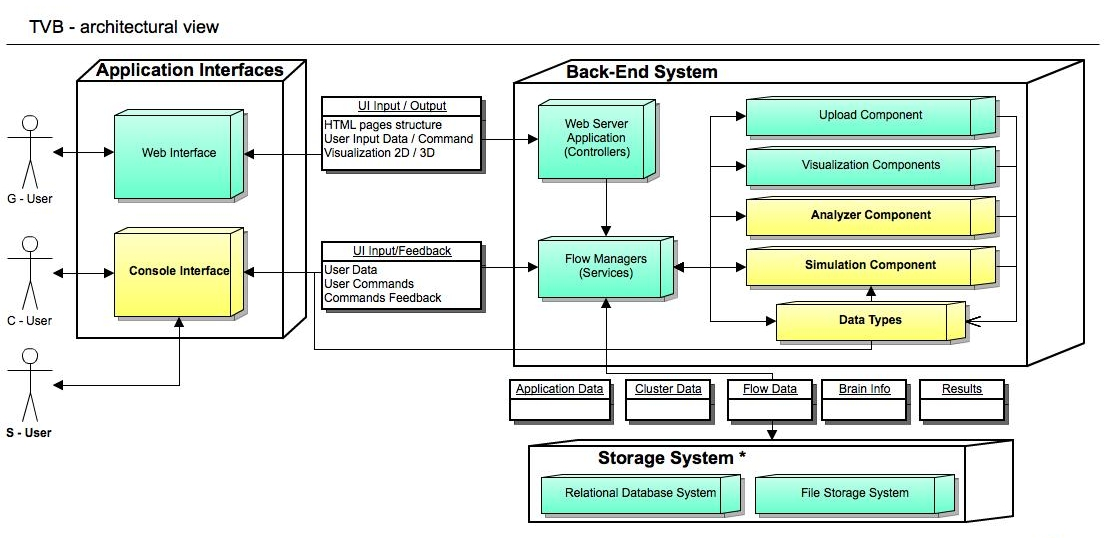
\includegraphics[width=0.90\textwidth]{images/architecture.jpg}
        \caption{\TVB architecture: 
        Yellow blocks are part of the Scientific Library of TVB, while the green blocks are part of TVB Framework.
        TVB provides two independent interfaces, depending on the interaction type wanted by the end-user (web or console).
        TVB Storage layer is compulsory for the web interface, but it can be switched on/off for the console interface.
         }
        \label{fig:architecture}
 \end{figure*}


	\subsection{TVB Scientific Library}

	\subsubsection{General description}

	\subsubsection{Datatypes}

\paragraph{Description and examples}

\note[lp]{From FIN paper:} TVB-datatypes are annotated data structures which
contain one or more data attributes and associated descriptive information, as
well as methods for operating on the data they contain. The definition of a
datatype is achieved using TVB's traiting system, which was inspired by the
traiting system developed by Enthought \cite{Enthought_2001} 

\note[lp]{The TVB-trait system might be worth described here?}

\note[lp]{Table 2 "TVB datatypes" of FIN article might be interesting here?}

In scientific Python code, it is conventional to provide arguments
of an algorithm as a "bare" array or collection there of, and sanity
checks of arguments proceed on the basis of array geometry, for example.
In \TVB, we consider a \textit{datatype} to be a full, formal description of 
an entity involved in an algorithm that would be part of \TVB. 
For example, the \texttt{Connectivity} datatype, which may elsewhere
be represented by a simple $N$ by $N$ NumPy array, is written as a class
in which one of the attributes, \texttt{weights} is a explicitly typed 
\texttt{FloatArray}, and the declaration of this type is complemented by
explicit label, default values, and documentation strings. 

\note[mw]{Add a listing showing this}.

Because an explicit goal of \TVB was to provide a user interface to each of the
datatypes and algorithms contained within, it is necessary at some point to
provide metadata. A \texttt{traits} system was developed, similar to that of
IPython or EPD, was developed, allowing for a attributes of a datatype class to
be written out with full metadata. An extensive set of existing building 
blocks are already provided from numeric types and arrays to lists, tuples, 
string, and dictionaries.

\note[mw]{Show description of a data type}

 When methods of such a class are invoked,
they may use the traited attributes directly, accessing either a default value
or one given during the instantiation of the object. Additionally, this allows
the web-based UI to introspect a class for all of its attributes and their
descriptions, to provide help in the interface. The explicit typing also allows
such classes to be nearly automatically mapped to SqlAlchemy \& HDF5 tables,
the combination of which provides persistence for datatypes when using the web
UI.  Lastly, because such metadata is used to build the docstring of a class,
the IPython user also may obtain extensive descriptions of attributes and
function arguments in the usual way. 

\note[lp]{The Connectivity datatype might be an example}


\subsection{TVB Framework}

	\subsubsection{General description}

The framework has been developed with generality and modularity in mind. It
provides a database back-end, workflow management and a number of features to
support collaborative work.  The central idea is data-oriented in a sense that
data are fed and stored into the system and can be transformed into another type
of data (including visualization) through the operation provided by an external
library (including TVB scientific library, but not restricted to it) that have
been \emph{adapted} to the framework. As a consequence, the two central concepts
are \emph{datatypes} i.e. types of data that can be handled in the framework and
\emph{adapters} i.e. processes that allow to interface/adapt external libraries
to  the datatypes handled by within the framework.

The framework also provides user interfaces: web-based graphical interface and
console interface for advanced user and developers.

Due to the generality of the framework, it relies on
the Python \emph{abstract classes} mechanism.
\note[lp]{From Python glossary:}
Abstract base classes complement duck-typing by providing a way to define
interfaces when other techniques like hasattr() would be clumsy or subtly wrong.

\subsubsection{Data Storage}

Data storage is managed using \emph{SQLAlchemy}
\texttt{http://www.sqlalchemy.org/} which provides a common interface for the
two proposed storage system: SQLite and PostgreSQL \note[lp]{or flat file
system?}.

\subsubsection{Adapters}

\paragraph{General description}

While datatypes provide a way of description what algorithms work with, 
sufficing for the typical user looking to write scripts against the
available libraries, the web-based UI requires algorithms to adhere to 
a generic interface, which is elsewhere referred to as the Adapter pattern.
Typically, this implies that a class is written that is able to describe
the collection to datatypes required and a single method to invoke the
algorithm.

Adapters are derived from the abstract class named \texttt{ABCAdapter} which
defines the common interface for the adapters with methods...

Several categories of adapters have been defined: 
\begin{itemize}
    \item \textit{analyzers} which allow the interface between libraries
        containing algorithm for the analysis of the data (wavelets, FastICA,
        etc.) and the TVB framework and datatypes.
    \item \textit{creators}
    \item \textit{exporters} 
    \item \textit{portlets} 
    \item \textit{simulator}
\item \textit{uploaders}: allow the upload of external data into TVB framework
    such as gifti files of plain csv files.
\item \textit{visualizers} \note[lp]{derived from the ABCDisplayer abstract class} allow
    to display the correct datatype.
\end{itemize}


\note[mw]{Show the adapter for FastICA}

Note that the adapters and datatypes are intended to provide full 
power and flexibility of the framework; when the simulator is invoked from
the web-based UI, it is done so through an \texttt{SimulatorAdapter} which,
despite being relatively complex, is datatypes all the way down.

It is reasonable to ask to what such a scheme offers over the more 
conventional approach of Python, where presumably it would have been
sufficient that each adapter consist of a class with an \texttt{\_\_init\_\_}
and \texttt{\_\_call\_\_} method, in the case of a function type. 
We note that because in the case of \TVB, the context in which an object
is used is more varied, e.g. not simply initialized but loaded through 
SqlAlchemy's ORM, and that the adapter is required to perform more tasks
than just initialization and invocation, e.g. provide expected shape of 
result, it was advantageous to create a distinct set of interfaces built
on the abstract base class framework provided by Python's standard library.

\paragraph{Adapting sklearn's FastICA}

\paragraph{Interfacing with MATLAB}

One of the well-known libraries for characterizing anatomical 
and functional connectivity is the Brain Connectivity Toolbox. Because
it is written in MATLAB, with maintainers who prefer MATLAB, we 
chose not to port routines of the library to Python but instead use
a MATLAB adapter which runs arbitrary MATLAB code. This generic
adapter works by generating a wrapper script for the MATLAB code, which
wraps the code in a try-except clause, and loads and saves the workspace
before and after execution, 
generating a workspace \texttt{.mat} file, invoking the MATLAB or Octave
executable, and loading the resulting workspace file. Despite invocation
of MATLAB being a relatively slow operation, this works fine in a single
user situation, and where Octave is available, it is quite fast. In the 
case that many operations are necessary, they can be batched into the 
same run.




\section{Simulator}
The simulator in TVB resembles popular neural network simulators in 
many fundamental ways, both mathematically and in terms of informatics 
structures, however we have found it necessary to introduce auxiliary
concepts particularly useful in the modeling of large scale brain 
networks. In the following, we will highlight some of the interesting
principles and capabilities of TVB's simulator and give rough characterization
of the execution time and memory required in typical simulations.

\subsection{Node dynamics}

	In TVB, nodes are not considered to be abstract neurons nor necessarily
	small groups thereof, but rather large populations of neurons. Concretely,
	the main assumption of the neural mass modeling approach in TVB is that
	large pools of neurons on the millimeter scale are strongly approximated
	by population level equations describing the major statistical modes of
	neural dynamics \cite{Freeman_1975book}. Often, averaging techniques are
	employed, though techniques retaining several modes have been developed
	\cite{Stefanescu_2008, Stefanescu_2011}. Such an approach is certainly not
	new; one of the early examples of this approach consist of the well known
	Wilson-Cowan equations \cite{Wilson_1973}. Nevertheless, there are
	important differences in the the assumptions and goals from modeling of
	individual neurons, where the goal may be to reproduce correct spike
	timing or predict the effect of  a specific neurotransmitter. A second
	difference lies in coupling: chemical coupling is often assumed to be
	pulsatile, or discrete, between neurons, whereas it is considered
	continuous. Typically the goal of neural mass modeling is to study the
	dynamics that emerge from the interaction of two or more neural masses and
	the network conditions required for stability of a particular
	spatiotemporal pattern. In the following, we shall  briefly discuss some
	of the models available in TVB.

	As we have noted, many neural mass models have been developed. One of
	the more prominent examples in the systems neuroscience literature is 
	that the Jansen-Rit model of rhythms and evoked responses arising from
	coupled cortical column \cite{Zetterberg_1978, Jansen_1995, Spiegler_2010}. 
	\note[mw]{Continue description}.
	\note[psl]{maybe see David et al, 2004 for better description of local connectivity in the Jansen and Rit model}
	Advantages of the Jansen-Rit model stem from the connection made
	between empirical studies of neural tissue and the model's parameters, 
	making it easier in certain cases to make concrete predictions about
	the relation between a dynamical regime and its neurobiological 
	mechanism. However, because the form of the model used often employs
	at least six dimensions, it is not always clear how to analyze or
	visualize. Lastly, the model requires frequent computation of exponentials,
	requiring considerable computational time. 

	For these reasons, it is often desirable to have a simpler mathematical 
	model, which may be reproduce the same qualitative phenomena as other 
	models, implemented with fewer and simpler equations. Such is the motivation
	for the generic two-dimensional oscillator model provided by TVB. 
	Model produces oscillations, damped, spike-like or 
	sinusoidal activations. While these alone are not interesting, they 
	permit the study of network phenomena, such as synchronization of rhythms
	or propagation of evoked potentials, while requiring less time to simulate.

	However, the modeler's goals may not lead to either the Jansen-Rit
	\cite{Jansen_1995, David_2003, David_2004} or generic 2D oscillator
	\cite{FitzHugh_1961, Nagumo_1962}, and several other mass models are
	provided by TVB: the previously mentioned Wilson-Cowan description of
	functional dynamics of neural tissue \cite{Wilson_1972}, the Kuramoto
	model describing synchronization \cite{Kuramoto_1975, Cabral_2011}, two
	and three dimensional mode-level models describing populations with
	excitability distributions \cite{Stefanescu_2011, Stefanescu_2008}, a
	reduction of the Wong and Wang model \cite{Wong_2006} as presented in
	\cite{Deco_2013} and a lumped version of Liley's model \cite{Liley_1999,
	Steyn-Ross_1999} model are among the available models in TVB.

	Again, should any of these be insufficient, a new model can be implemented
	with minimal effort by subclassing a base \texttt{Model} class and
	providing a  \texttt{dfun} method to compute the right hand sides of the
	differential  equations. Please refer to the \url{https://github.com/the-
	virtual-brain/scientific_library/tree/trunk/contrib/simulator/models} for
	examples. There, models found in the work of 
	\cite{Larter_1999, Breakspear_2003, Morris_1981, Hindmarsh_1984, Brunel_2001}
	have been implemented.

\subsection{Network structure}

	The network of neural masses in TVB simulations directly follows from  a
	pair of geometrical constraints on cortical dynamics. The first is the
	large-scale white matter fibers that form a non-local and heterogeneous
	(translation variant) connectivity, either measured by anatomical tracing
	(CoCoMac\ref{CoCoMac}) or diffusion-weighted imaging \cite{Hagmann_2008,
	Honey_2009, Bastiani_2012}. The second is that of horizontal projections
	along the surface, which are modeled through a translation invariant
	\note[sk]{Not technically true, using singular parameters will produce
	this but that's only a limited subset of the capability, spatially
	inhomogeneous parameters are supported -- thus being more general than the
	restricted case of translational invariance} connectivity kernel,
	approximating a neural field.

	\subsubsection{Large-scale connectivity}

	The large-scale region level connectivity at the scale of centimeters,
	resembles more a traditional neural network than a neural field in that
	neural space is discrete,  each node corresponding to a neuroanatomical
	region of interest, such as V1, etc. It is at this level that inter-regional 
	time delays play a large role, whereas the time delays due to 
	lateral, local projections are subsumed under the dynamics of the node.

	It is often seen in the literature that the inter-node coupling functions
	\textit{are} part of the node model itself. In TVB, we have instead 
	chosen to factor such models into the intrinsic neural mass dynamics, where each 
	neural mass's equations specify how connectivity contributes to the
	node dynamics, and the coupling function, which specifies how the activity
	from each region is mapped through the connectivity matrix. Common coupling 
	functions are provided such as the linear, difference and periodic functions
	often used in the literature.

	\subsubsection{Local connectivity}

	The local connectivity of the cortex at the scale of millimeters provides
	a continuous 2D surface along horizontal projections connect 
	cortical columns. Such a structure has previously been modeled by
	neural fields \cite{Amari_1977, Jirsa_1997, Liley_1999}. In TVB, a cortical mesh, 
	as obtained from structural MRI data and simplified, provides a spatial 
	discretization on which neural masses are placed and connected with a
	local connectivity kernel, itself only a function of the geodesic distance
	between the two masses, and this is considered to provide an
	approximation of a neural field, depending on the properties
	of the mesh and the imaging modalities that sample the activity simulated
	on the mesh \cite{Spiegler_2013}. 
	\note[sk]{The implementation of the local connectivity kernel is such
	that is can be re-purposed as a discrete Laplace-Beltrami operator,
	allowing for the implementation of true neural-field models that 
	use a second-order spatial derivative as their explicit spatial term.}

	TVB currently provides several connectivity kernels, of which a Gaussian
	is one. Once a cortical surface mesh 
	and connectivity kernel and its parameters are chosen, the geodesic
	distance (i.e. the distance along the cortical surface) is evaluated
	between all neural masses \cite{Mitchell1987}, and a cutoff is chosen
	past which the kernel falls to 0. This results in a sparse matrix that 
	is used during integration to implement the approximate neural field. 
	\note[psl]{The Laplacian kernel is not implemented yet.}

\subsection{Integration of stochastic delay differential equations}

	In order to obtain numerical approximations of the network model 
	described above, TVB provides both deterministic and stochastic
	Euler and Heun integrators,
	following recent literature on numerical solutions to stochastic
	differential equations \cite{Kloeden_1995,Mannella_2002,Mannella_1989}.

	While the literature on numerical treatment of delayed or 
	stochastic systems exists, it is less well known how to treat 
	the presence of both. For the moment, the methods implemented by TVB
	treat stochastic integration separately from delays. 
	This separation conincides with a modeling assumption that in
	TVB the dynamical phenomena to be studied are largely determined
	by the interaction of the network structure and neural mass dynamics, 
	and that stochastic fluctuations do not fundamentally reorganize the
	solutions of the system \cite{Ghosh_2008,Deco_2009,Deco_2011,Deco_Senden_2012}.

	Due to such a separation, the implementation of delays in the
	regional coupling is performed outside the integration step,
	by indexing a circular buffer containing the recent simulation 
	history, and providing a matrix of delayed state data to the 
	network of neural masses. While the number of pairwise
	connections rises with $n_{region}^2$, where $n_{region}$ is
	the number of regions in the large-scale connectivity, 
	a single buffer is used, with a shape
	$(horizon, n_{cvar}, n_{region})$ where $horizon = max(delay) + 1$,
	and
	$n_{cvar}$ is the number of coupling variables. Such a scheme helps 
	lower the memory requirements of integrated the delay equations.

\subsection{Forward solutions}

	A primary goal of TVB is not only to model neural activity itself
	but just as importantly the imaging modalities common in human 
	neurosciences, using so-called forward solutions, which allow for
	the projection of neural activity into sensor space. To account
	parsimoniously for other ways in which simulated data might be saved, 
	such as simple temporal averaging, we refer to each of these simply as 
	\textit{Monitors}, which take as input neural activity and 
	output a particular projection thereof. In most cases, this 
	takes the discrete-time form of

	\[ \hat{y}[j, t] = \sum_{i=1, \tau=1}^{N_W, N_k} W[j, i] K[\tau] y[i, t-\tau] \]

	\noindent where $y[i, t]$ is the amplitude of the $i^{th}$ neural mass at time
	$t$, $K[\tau]$ is a temporal kernel, and $W[j, i]$ is a spatial kernel,
	usually projecting the state variable of interest of the $i^{th}$ 
	neural mass to the $j^{th}$ sensor. 

	Where necessary for computational reasons, monitors employ more than 
	one internal buffer. The fMRI monitor is one 
	example: given a typical sampling frequency of simulation may be upward of 
	64 kHz, and the haemodynamic response function may last several seconds, 
	requiring many gigabytes of memory for the fMRI monitor alone. Given that 
	the time-scale of simulation and fMRI differ by several orders of magnitude, 
	the subsequent averaging and downsampling is justified. 

	In the cases of the EEG and MEG monitors, $K$ implements a simple
	temporal average, and $W$ consists of a so-called lead-field matrix as typically
	derived from a combination of structural imaging data of the patient 
	and the locations and orientations of the neural sources and the locations
	and orientions of the EEG electrodes and MEG gradiometers and magnetometers. 
	As the development and implementation of such lead-fields is well developed
	elsewhere \cite{Jirsa_2002,Nolte2003,Gramfort_2010}, TVB provides access
	to the well-known OpenMEEG package, however, the user is free to provide 
	his or her own.

\subsection{Performance}

	A primary goal of the simulator is to be available as a pure Python package,
	and secondarily, to be fast enough. We have not found it useful to 
	develop theoretical estimates of the time and space complexity of the 
	algorithms, given that much of the heavy lifting is already done in native
	code by NumPy and other standard libraries. Instead, 
	in the following, we profile a set of eight characteristic simulations
	on both memory use, specifically the heap size as measured by Valgrind's 
	\texttt{massif} tool \cite{valgrind2007}, and function timing as measured by the 
	\texttt{cProfile} module of the standard library. 
	
	Measurements were
	performed on an HP Z420 workstation, with a single Xeon E5-1650
	six-core CPU running at 3.20 GHz, L1-3 cache sizes 384 KB, 1536 KB
	and 12 MB respectively, with main memory 4 x 4 GB DDR3 at 1600 Mhz,
	running Debian 7.0, with Linux kernel version 3.2.0-4-amd64. 
	The 64-bit Anaconda Python distribution was used with additional Accelerate
	pacakge which provides acceleration of common routines based on the 
	Intel Math Kernel Library. A Git checkout of the trunk branch of TVB 
	was used with SHA 6c644ab3b5.

	Eight different simulations were performed corresponding to the combinations of
	either the generic 2D oscillator or Jansen-Rit model, region-only
	or use of cortical surface, and two conduction speeds, $v_c = 2.0$ and
	$v_c = 20.0$ (m/s). In each case, a temporal average monitors at 512 Hz
	is used, and the results are discarded. The region-only simulation was
	run for a second while the surface simulation was run for 100 ms. 

	\note[mw]{Table of profiling results to go here. Profiling has been done, 
	curating results now..}

\subsection{Acceleration with C \& CUDA}

	Several of the core components (integrators, mass models, coupling
functions) have targeted towards a C source code backend, which has
allowed for the compilation of simulations to native code loaded 
either as a shared library accessed via the \texttt{ctypes} modules
or as CUDA kernels accessed via the PyCUDA \cite{PyCUDA}. 
While such an approach may provide speed ups, they depend on the
presence of a C compiler and, in the case of GPU, the CUDA toolkit and
a compatible graphics card, and in the future, prepackaged versions of TVB
will include precompiled objects for most kinds of simulations. 

A common approach in Python numerical libraries to eliminating Python
overhead is to rewrite code in Cython. However, an explicit goal in 
the case of TVB was
to employ thread parallelism on the GPU, with C code as a fallback 
possibility. 

The approach used in compiling a simulation to native code thus takes advantage
of the fact that code that must be generated for CUDA is quite similar to C,
and thus a generic template abstracts much of the boilerplate between the two.
For each part of the simulator, a generic function is customized with a class
specific kernel; for example, in the case of a neural mass model, we have in
the Python class

\begin{lstlisting}[caption={The Generic2dOscillator listing},
	       label={lst:g2dOscil}]
class Generic2dOscillator(Model):
    tau = FloatArray(...)
    # etc.

    device_info = model_device_info(
	pars=[tau, a, b, c, d, I],
	kernel="""
	float tau  = P(0)
	    , a    = P(1) ; // etc

	// state variables
	    , v    = X(0)
	    , w    = X(1)

	// aux variables
	    , c_0  = I(0)   ;

	// derivatives
	DX(0) = d * 
	(tau * (w - v*v*v + 3.0*v*v + I + c_0));
	DX(1) = d * 
	((a + b*v + c*v*v - w) / tau);
	"""
    )
\end{lstlisting}

\noindent where the device\_info attribute is used to specify how the
class's mathematical description fits into the general model function:

\begin{lstlisting}[caption={The Listing},label={lst:wrapper}]
/* wrapper for model specific code computing RHSs of diff-eqs */
__device__
void model_dfun(
  float * _dx, float *_x, float *mmpr, float *input)
{
#define X(i) _x[n_thr*i]
#define DX(i) _dx[n_thr*i]
#define P(i) mmpr[n_thr*i]
#define I(i) input[i]

    // begin model code
    \$model_dfun
    // end model specific code

#undef X
#undef DX
#undef P
#undef I
\end{lstlisting}

\noindent where the C preprocessor defines allow the model specific
kernel to easily reference the correct parts of the multidimensional 
per-thread arrays (in the case of the GPU). 

 \begin{figure}
	{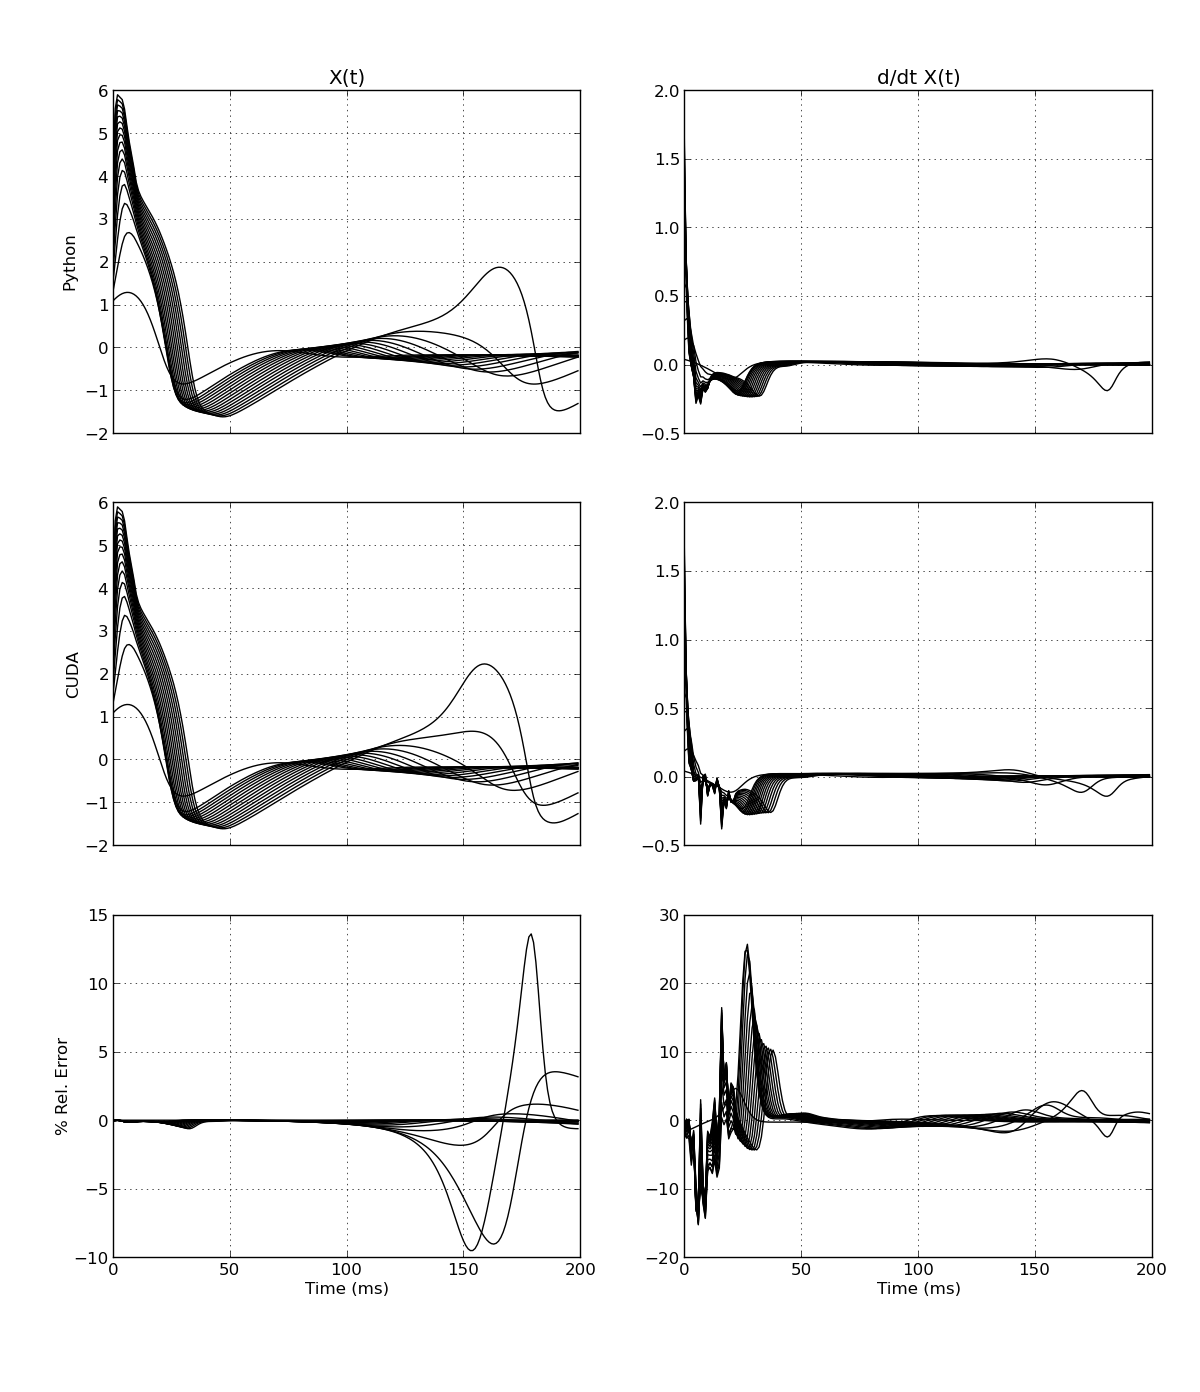
\includegraphics[width=0.48\textwidth]{images/gpu_dxdt.png}}
	\caption{
	Right A typical parameter space exploration, 32 x 32 grid of
	coupling strength (y-axis) v. neural excitability (x-axis).
	This grid of simulations was run on both TVB's Python/NumPy
	implementation and the new GPU backend for 200 ms simulation
	time with otherwise default parameters. The former took ~2
	hours and the latter ~ 1 min. Left Quantitative comparison of
	solutions and instantaneous derivatives is shown for an even
	sampling of the parameter space across k where a = -2, because
	this slice showed the most error on the GPU. 	
	}
	\label{fig:gpu_dxdt}
\end{figure}

 \begin{figure}
	{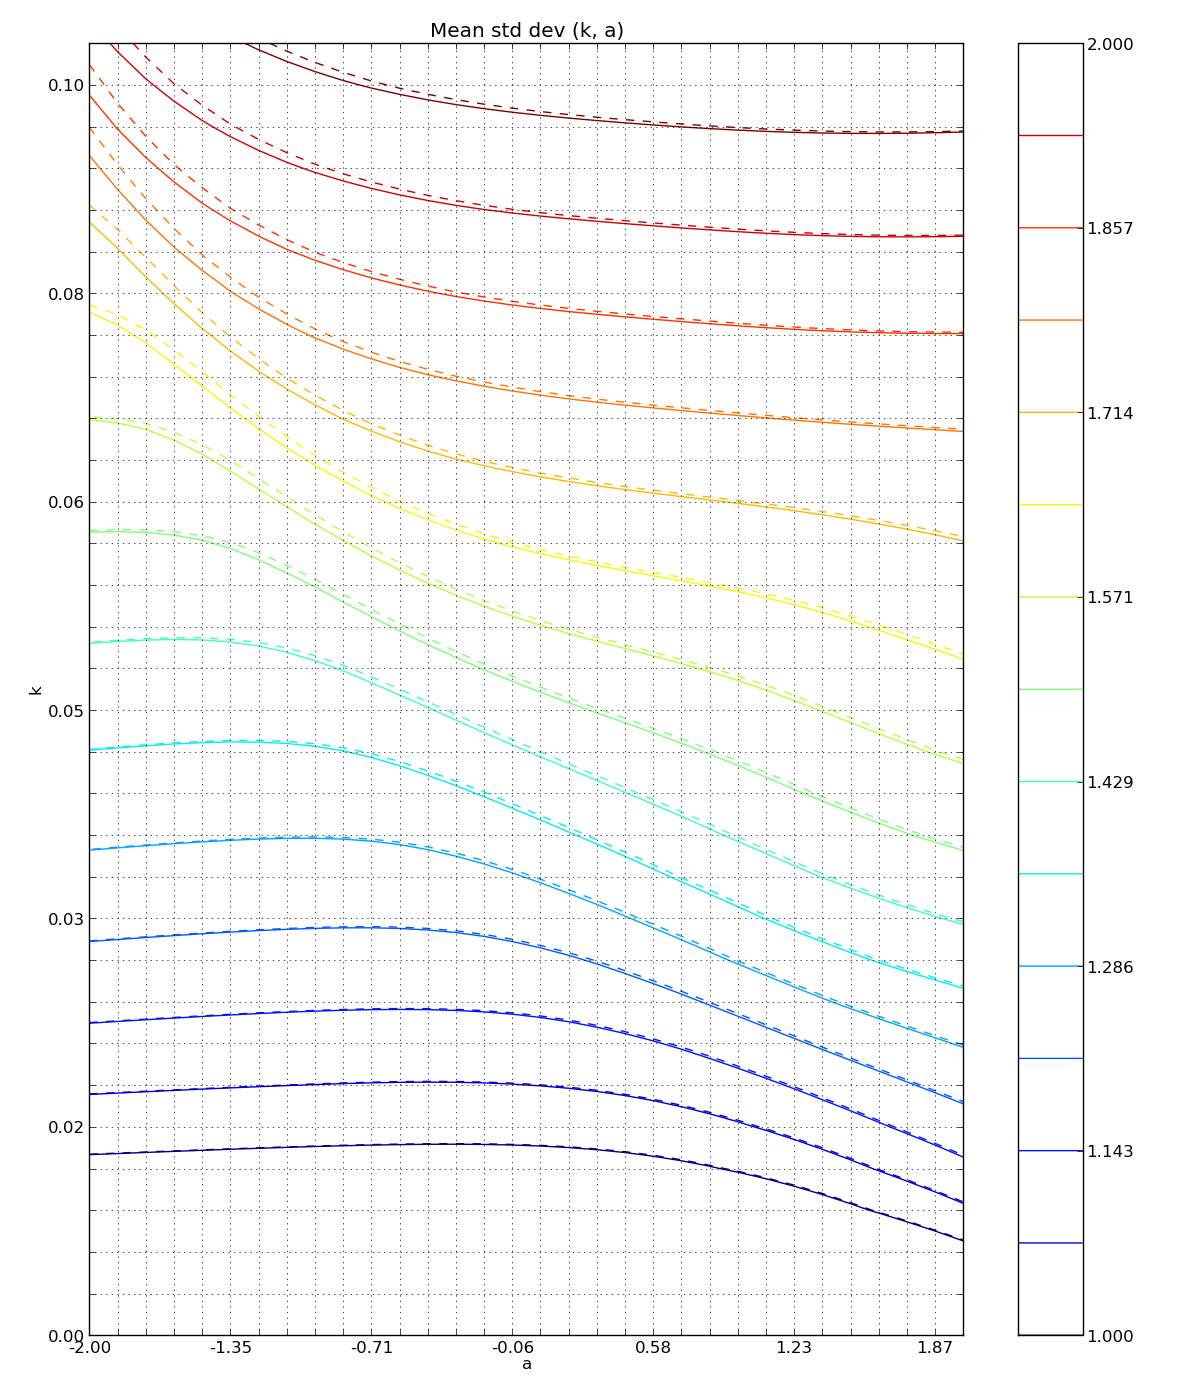
\includegraphics[width=0.48\textwidth]{images/gpu_pse.png}}
	\caption{}
	\label{fig:gpu_pse}
\end{figure}

\note[sk]{One figure or two, re captions}

\note[sk]{Specify hardware (GPU/CPU) and whether Numpy is mkl-linked, to 
    provide a more solid foundation for timing comparisons...}

\note[sk]{It would be interesting to see a longer run (say a few seconds)
    to show if/how-quickly the error grows...}

As can be seen in the listing \note[sk]{can listings be numbered and
labelled...}\note[lp]{Done see example and edit}, the calculations
in native code are performed with 32-bit floating point numbers, and it
is reasonable to ask if this is numerically accurate. In Fig 
\ref{fig:gpu_pse}, we present a parameter space exploration performed with
both the pure Python NumPy simulator and the GPU simulator, showing the 
isocontours of average standard deviation in the parameter space. Some
deviation can be identified visually in parts of the parameter space, and
in in Fig \ref{fig:gpu_dxdt}, we show in more detail time series of 
the Python and GPU solutions.

 \begin{figure}
	{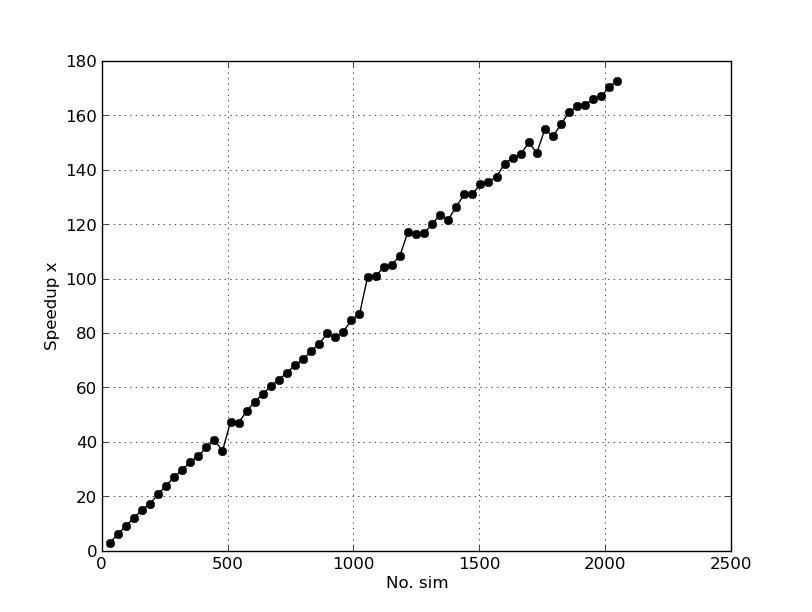
\includegraphics[width=0.48\textwidth]{images/gpu_acceleration.png}}
	\caption{}
	\label{fig:gpu_acceleration}
\end{figure}

This approach allows significant acceleration of parameter sweeps in the
case of the GPU by taking
advantage of the fact that in many cases, only numerical values vary
between different threads and not memory access patterns. Where one of the
dimensions of a parameter sweep implies changing memory access patterns, 
for example conduction speed, it is advantageous to reorder the parameters,
so that such memory varying parameters only change between grids of GPU
threads and not within.

In Fig \ref{fig:gpu_acceleration}, we plot the speedup brought by the GPU
over the Python NumPy simulator as a function of the number of simulations 
performed simulataneously on the GPU.




\section{User Interaction}

\note[mw]{Focus more on scripting}

\subsection{Web Interface}

	\subsubsection{Projects, Users \& Data}

	\subsubsection{Simulator Interface}
	
	\subsubsection{Visualizers \& Analysis}

	\subsubsection{Connectivity Tool}

\subsection{Python scripting}

	\subsubsection{Hello Brain}
		\note[mw]{A quick, basic example}

	\subsubsection{Anatomy of a simulation}
		\note[mw]{Maybe cherrypick from the tutorial Stuart wrote}

	\subsubsection{Custom connectivity}
		\note[mw]{Perhaps you just want a simple network?}
		
	\subsubsection{Online feedback}
		\note[mw]{Or modify a parameter as a function of activity?}


\section{Future Work}

- testing
- documentation


On going work on the simulator includes

\begin{enumerate}
	\item Code generation in the simulator to compile specifications to native
		code running independently of TVB or on the GPU.
	\item MATLAB interface
	\item Spatial derivatiaves (?) 
\end{enumerate}

As previously stated, the primary goal of the \TVB is to provide the means
to pass all the way from structural imaging data to dynamic imaging. We
aren't there yet, as several pieces still require scientific consensus 
and standards. Notably, 

\begin{enumerate}
	\item DTI pipeline
	\item Connectome Project
	\item Structural imaging processing via FreeSurfer (pySurfer, NiPy, etc.)
	\item NeuroML project	
\end{enumerate}


In the near future, our informatics efforts outside of these areas will
focus on making the platform accessible and demonstrating the validity
of the simulations with respect to empirical data.



\section*{Acknowledgments}
 Several authors have also participated in the development of TVB. They are cited in the
\texttt{AUTHORS} file in TVB distribution and deserve also our warm acknowlegments. LP whishes to thank specifically Y.~Manhoun for his implication in the conception and development of the first prototype of the TVB architecture. The research reported herein was supported by the  Brain Network Recovery Group through the James S. McDonnell Foundation and the FP7-ICT BrainScales. PSL is supported by a doctoral fellowship from Ministere de la Recherche.

\bibliographystyle{apalike}
\bibliography{bib}

\end{document}

